\begin{figure*}
\centering
\begin{subfigure}{0.8\textwidth}
\centering
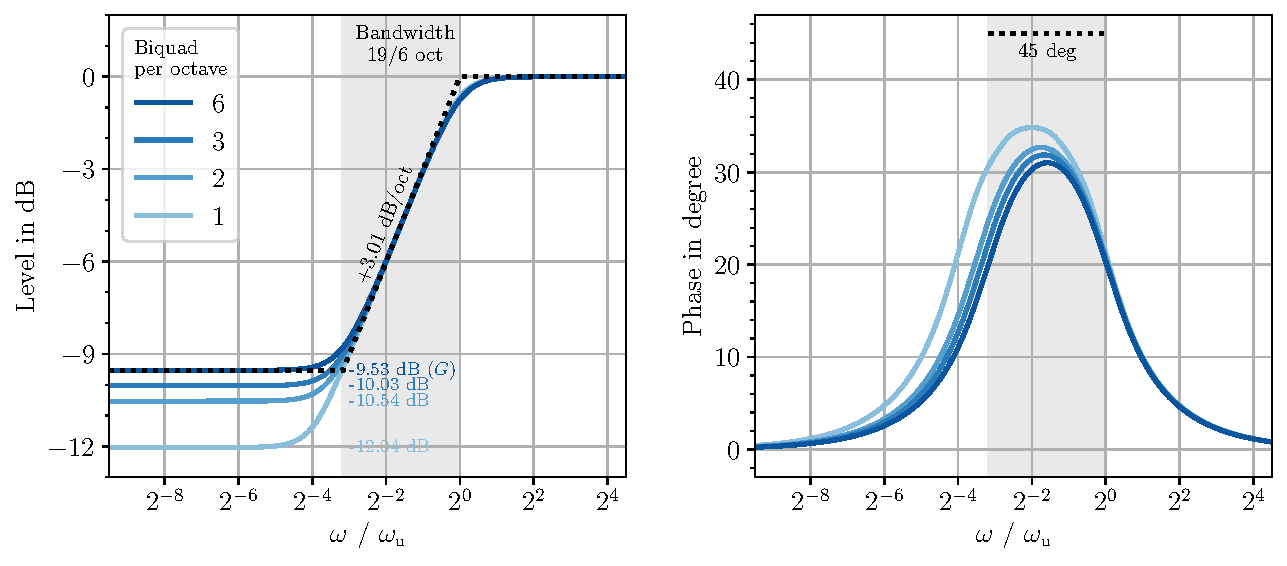
\includegraphics[width=\textwidth]{../graphics/gain-error.pdf}
\caption{Slope $\chi = 10\lg(2)\approx +3.01$ dB/oct and shelving
level $G=-\frac{19}{6} \cdot \mathrm{oct} \, \chi \approx - 9.53$ dB yields a bandwidth
of $\beta = 19/6$ octaves.
The resulting shelving level deviates from $G$ for less than $N_O = 6$
biquads per octave.}
\label{fig:gain-error}
\end{subfigure}
\\
\begin{subfigure}{0.8\textwidth}
\centering
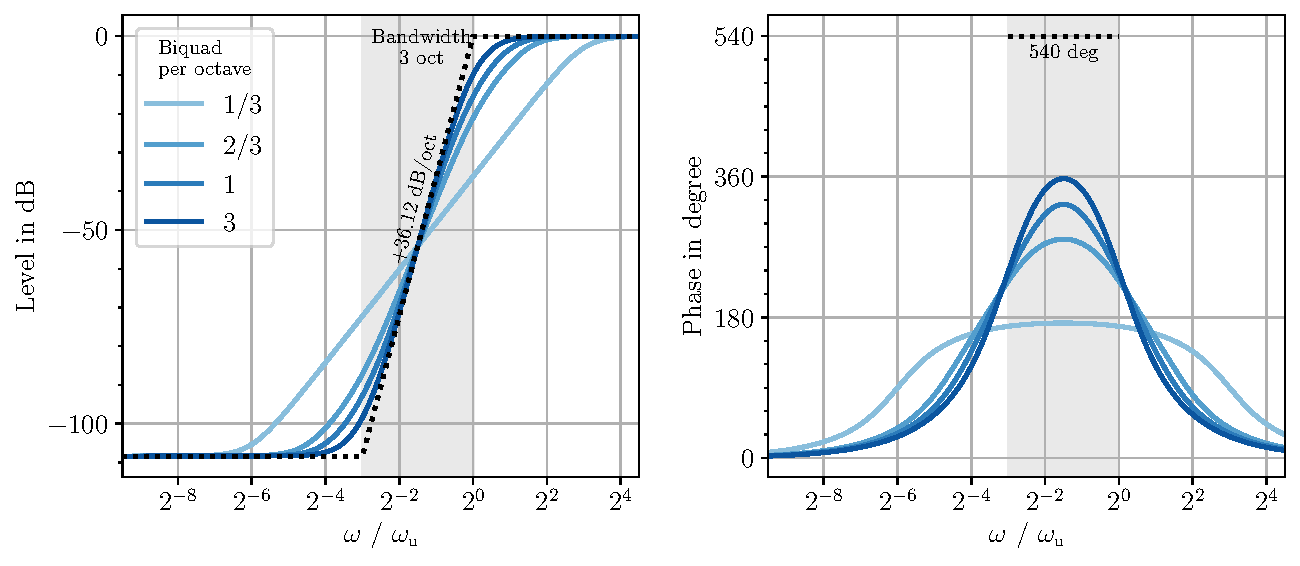
\includegraphics[width=\textwidth]{../graphics/slope-error.pdf}
\caption{Slope $\chi = 120 \lg(2) \approx +36\,\mathrm{dB/oct}$ and bandwidth $\beta=3$
octaves yields shelving level $G=-360\lg10(2) \approx -108$ dB.
The resulting bandwidth deviates from $\beta$ when deploying less than $N_O = 3$
biquads per octave.
}
\label{fig:slope-error}
\end{subfigure}
\\
\begin{subfigure}{0.8\textwidth}
\centering
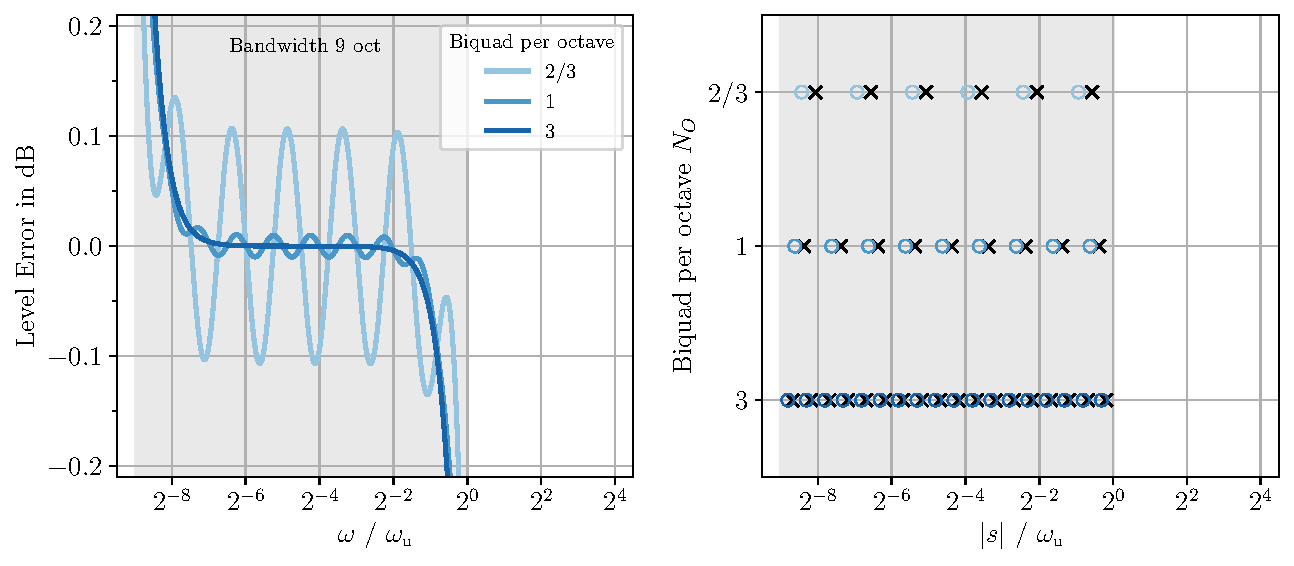
\includegraphics[width=\textwidth]{../graphics/ripple-and-zp-frequency.pdf}
\caption{$\beta=9$ oct,
$G=-10\lg(2)\approx -3$ dB yields
$\chi =  \frac{10}{9}\lg(2) \approx + 0.3345$ dB/oct.
Left: $20\lg|H(\omega)|-20\lg|H_\mathrm{ideal\,slope}(\omega)|$.
Right: distribution of poles (x) and zeros (o).}
%depending on number of biquads
%per octave.
\label{fig:ripple-and-zp-frequency}
\end{subfigure}
%
\caption{Shelving filter cascade frequency responses.
%
Limitations of the filter design method occur due to the discrete number of
cascaded biquads to represent a fractional-order filter slope.
}
\label{fig:shelving_filter_error_cases}
\end{figure*}
